\documentclass[a4paper, 12pt]{exam}
\usepackage[T1]{fontenc} 
\usepackage{amsmath}
\usepackage{amssymb}
\usepackage{enumerate}
\usepackage{bm}
\usepackage{advdate}
\usepackage{datetime}
\usepackage[mathcal]{eucal}
\usepackage{dsfont}
\usepackage{listings}
\usepackage{xcolor}
\usepackage{graphicx}
\definecolor{codegreen}{rgb}{0,0.6,0}
\definecolor{codegray}{rgb}{0.5,0.5,0.5}
\definecolor{codepurple}{rgb}{0.58,0,0.82}
\definecolor{backcolour}{rgb}{0.95,0.95,0.92}

\lstdefinestyle{mystyle}{
	backgroundcolor=\color{backcolour},   
	commentstyle=\color{codegreen},
	keywordstyle=\color{magenta},
	numberstyle=\tiny\color{codegray},
	stringstyle=\color{codepurple},
	basicstyle=\ttfamily\footnotesize,
	breakatwhitespace=false,         
	breaklines=false,                 
	captionpos=b,                    
	keepspaces=true,                 
	numbers=left,                    
	numbersep=5pt,                  
	showspaces=false,                
	showstringspaces=false,
	showtabs=false,                  
	tabsize=2
}
\lstset{style=mystyle}
\usepackage{url}
\newdate{issuedate}{23}{10}{2020}
\newdate{duedate}{6}{11}{2020}

% \newcommand{\duedate}[1][14]{%
% \begingroup
% \AdvanceDate[#1]%
% \today%
% \endgroup
% }%

\usepackage[thehwcnt=2]{iidef}
\thecourseinstitute{Tsinghua-Berkeley Shenzhen Institute}
\thecoursename{Learning From Data}
\theterm{Fall 2020}
\makeatletter
\newcommand{\firstblock}{programming_policies}
\makeatother

\begin{document}
	
	\pagestyle{headandfoot}
	\runningheadrule
	
	
	\newcounter{psctr}
	\setcounter{psctr}{1} % set to the times of problem
	
	\runningheader{Programming Assignment \thepsctr}
	{\textsc{Learning from Data}}
	{ Page \thepage\ of \numpages}
	\firstpagefooter{}{}{}
	\runningfooter{}{}{}
	
	
	\newcounter{Sequ}
	\newenvironment{Sequation}
	{\stepcounter{Sequ}%
		\addtocounter{equation}{-1}%
		\renewcommand\theequation{S\arabic{Sequ}}\equation}
	{\endequation}
	%\topskip0pt
	
	% \vspace*{\fill}
	\centering
	
	% \vspace{0.3em}
	\centering
	\renewcommand{\thequestion}{\arabic{psctr}.\arabic{question}}
	\hwname{Programming Assignment}
	\courseheader
	\begin{flushleft}
		\textbf{Issued:} \displaydate{issuedate} \hfill
		\textbf{Due:} \displaydate{duedate} 
	\end{flushleft}
	
	\hrule 
	
	\input{\firstblock}
	
	%\pointname{}
	%\vspace{\footskip}
	\vspace{1em}
	
	
	%\pointname{}
	%\vspace{\footskip}
	%\vspace{1em}
	
	\begin{questions}
		\question (5 points) \emph{Automatic differentiation} In class, we have learned to build a neural network, we need to implement the forward
		and backward propagation of given network model. This underlining mechanism is also called Automatic differentiation, autodiff for short.
		Following the convention of popular neural network library. We call an object with the ability of autodiff \texttt{tensor}.
		To explain autodiff operation of tensor, we take a single variable function $f(a) = a^2 + 3a$ for an example. Then the tensor object
		\texttt{a,p,s,f\_a} are defined as follows:
		\begin{lstlisting}[language=Python]
			a = tensor()
			p = product(a, a)
			s = scale(a, 3)
			f_a = add(p, s)
		\end{lstlisting}
		The forward propagation evaluates the function value $f$ for given $a$ and can be decomposed into the following computational graph.
		\begin{figure}[!ht]
			\centering
			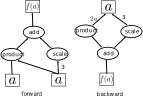
\includegraphics[width=6cm]{auto.eps}
		\end{figure}
		To implement this forward pass, we only need to implement \texttt{add}, \texttt{product}, \texttt{scale} operators and use the following pseudo Python code
		to evaluate $f(a)$ at $a=1.2$:
		\begin{lstlisting}[language=Python]
		f_a.eval(1.2) = s.eval(1.2) + p.eval(1.2)
		s.eval(1.2) = 3 * a.eval(1.2)
		p.eval(1.2) = a.eval(1.2) * a.eval(1.2)
		\end{lstlisting}
		The backward pass of $f(a)$ computes the derivative of $f$ about $a$, also illustrated in the above computational graph.
		\begin{lstlisting}[language=Python]
		a.back(f_a) = p.diff(a) * p.back(f_a) + s.diff(a) * s.back(f_a)
		p.back(f_a) = f_a.diff(p) * f_a.back(f_a)
		s.back(f_a) = f_a.diff(s) * f_a.back(f_a)
		\end{lstlisting}
		where \texttt{x.back(x)} is defined as identity as a convention since there is no back operation starting from self.
		The \texttt{diff} method of each tensor object computes the derivative about the adjacent variable.
		For example, \texttt{p.diff(a) = 2 * a}, \texttt{s.diff(a) = 3} etc.
		
		For multiple variable functions, the idea is the same as above but caution is needed for dimension coherence in matrix multiplication.
		
		Please implement Automatic differentiation for rank 2 tensor (matrix) based on coding template. To be more specific, you need to implement
		the atomic tensor object \texttt{product}, \texttt{scale}, \texttt{sigmoid} and some derived tensor object. We call a tensor object
		atomic if the method \texttt{eval} and \texttt{diff} should be implemented, while a derived tensor can be treated as composition of
		atomic tensor object.
		
		Hint: For rank 0 tensor (scalar) or rank 1 tensor (vector), we can treat
		them as special rank 2 tensor.
		
		\question (5 points) \emph{Multilayer perceptron} You have learned Ridge Regression and softmax regression, which can be treated
		as special kind of multilayer perceptron. There are no hidden layers on these regression model.
		
		\begin{equation*}
		l(\theta)= \sum_{i=1}^m y^{(i)} \log h_{\bm{\theta}}(\bm{x}^{(i)}) + (1-y^{(i)})\log(1-h_{\bm{\theta}}(\bm{x}^{(i)})) \textrm{ where } h_{\bm{\theta}}(\bm{x}) = \frac{1}{1+\exp(-\bm{\theta}^T \bm{x})}
		\end{equation*}
		We can use Newton's method to find the optimal $\bm{\theta}$, which has the following update scheme for $\bm{\theta}$:
		\begin{equation*}
		\bm{\theta}_{t+1} \leftarrow \bm{\theta}_t - H^{-1} \nabla_{\bm{\theta}} \mathcal{L}(\bm{\theta})|_{\bm{\theta}_t}
		\end{equation*}
		where $H$ is the Hessian matrix for the likelihood function $\mathcal{L}$.
		The scheme can be written in compact form as:
		\begin{equation*}
		\bm{\theta}_{t+1} = \bm{\theta}_t + (X^TRX)^{-1} X^T(\bm{y}-\bm{\mu}), \textrm{ where } \mu_i = h_{\bm{\theta}_t}(\bm{x}^{(i)}) \textrm{ and } R_{ii} = \mu_i ( 1 - \mu_i)\quad\footnote{$R$ is a diagonal matrix}
		\end{equation*}
 		Using Newton's method to fit the logistic model is also called {\em iterative reweighted least sqaures} (IRLS).
		
		Please implement IRLS by completing the code in \textbf{logistic\_regression.py}.
		
	\end{questions}
	
	
	\nocite{*}
	\begin{flushleft}
		\textbf{Notice}: \\
		\begin{enumerate}
			\item Use matrix operations other than loops for efficiency. If the running time of Auto-Grading steps exceeds 5 minutes, you will get point deductions.
			\item You are expected to only use \texttt{numpy} packages to implement the algorithms.
			\item All questions assume that the data are centered around zero. Therefore, you do not need to train the extra bias parameter in your code.
		\end{enumerate}
	\end{flushleft}
	
	%\bibliographystyle{plain}
	%\bibliography{ref}
	%\begin{thebibliography}{9}
	%	\bibitem{ridge} \href{https://ncss-wpengine.netdna-ssl.com/wp-content/themes/ncss/pdf/Procedures/NCSS/Ridge_Regression.pdf}{Ridge Regression}
	%	\bibitem{tutorial} \href{https://www.datacamp.com/community/tutorials/tutorial-ridge-lasso-elastic-net}{Regularization: Ridge, Lasso and Elastic Net}
	%\end{thebibliography}
\end{document}